\documentclass[10pt,landscape,a4paper]{article}
\usepackage[utf8]{inputenc}
\usepackage[ngerman]{babel}
\usepackage{tikz}
\usetikzlibrary{shapes,positioning,arrows,fit,calc,graphs,graphs.standard}
\usepackage[nosf]{kpfonts}
\usepackage[t1]{sourcesanspro}
%\usepackage[margin=0.05in]{geometry}
%\usepackage[lf]{MyriadPro}
%\usepackage[lf,minionint]{MinionPro}
\usepackage{multicol}
\usepackage{wrapfig}
\usepackage[top=0.2mm,bottom=2mm,left=1mm,right=1mm]{geometry}
\usepackage[framemethod=tikz]{mdframed}
\usepackage{microtype}
\usepackage{bbold}
\usepackage{wrapfig}
\usepackage{dsfont} % For mathbb{1}
\usepackage{amsmath}

% START CHEATSHEET TEMPLATE

\usepackage[default]{raleway}
\usepackage{fontawesome}
\usepackage[T1]{fontenc}

\usepackage{hyperref}
\usepackage{enumitem}
\setlist[enumerate]{itemsep=0mm}
\usepackage{lipsum}

\usepackage{xcolor}
\definecolor{customcolor}{HTML}{b5e9ff}
\definecolor{alert}{HTML}{CD5C5C}
\definecolor{w3schools}{HTML}{4CAF50}
\definecolor{subbox}{gray}{0.60}
\definecolor{codecolor}{HTML}{000000}
\colorlet{xx}{customcolor}

\usepackage{paralist}


%--------------------------Editor mode.

\usepackage
[citestyle=authoryear,
sorting=nty,	  		%Sorts bibliography by year, name, title
autocite=footnote, 		%Autocite command generates footnotes
autolang=hyphen, 		
mincrossrefs=1, 	
backend=biber]
{biblatex}

\DeclareFieldFormat{postnote}{#1}
\DeclareFieldFormat{multipostnote}{#1}
\DeclareAutoCiteCommand{footnote}[f]{\footcite}{\footcites}

\bibliography{literature}
%----------------------------------------
%--------------------------------------------------------------------------------
\usepackage{tcolorbox}

\tcbuselibrary{most,listingsutf8,minted}

\tcbset{tcbox width=auto,left=1mm,top=1mm,bottom=1mm,
right=1mm,boxsep=1mm,middle=1pt}

\newenvironment{mycolorbox}[2]{%
\begin{tcolorbox}[grow to left by=-1em,grow to right by=-1em,capture=minipage,fonttitle=\large\bfseries, enhanced jigsaw,boxsep=1mm,colback=#1!30!white,on line,tcbox width=auto, toptitle=0mm,colframe=#1,opacityback=0.7,nobeforeafter,title=#2]%
}{\end{tcolorbox}\\[0.2em]}

\newenvironment{subbox}[2]{%
\begin{tcolorbox}[capture=minipage,fonttitle=\normalsize\bfseries, enhanced jigsaw,boxsep=1mm,colback=#1!30!white,on line,tcbox width=auto,left=0.3em,top=1mm, toptitle=0mm,colframe=#1,opacityback=0.7,nobeforeafter,title=#2]\footnotesize %
}{\normalsize\end{tcolorbox}\vspace{0.1em}}

\newenvironment{multibox}[1]{%
\begin{tcbraster}[raster columns=#1,raster equal height,nobeforeafter,raster column skip=1em,raster left skip=1em,raster right skip=1em]}{\end{tcbraster}}

\newenvironment{textbox}[1]{\begin{mycolorbox}{customcolor}{#1}}{\end{mycolorbox}}

%-------------------------------
\newtcblisting{codebox}[2]{colback=codecolor!5,colframe=codecolor!80!black,listing only, 
minted options={numbers=left,style=tcblatex,fontsize=\scriptsize,breaklines,autogobble,linenos=false,numbersep=2mm},
left=4mm,enhanced,boxsep=1pt,left=2pt,right=1pt,top=0pt,bottom=0pt,
title=#2, fonttitle=\bfseries,
listing engine=minted,minted language=#1}

%--------------------------------------------------------------------------------
\newcommand{\punkti}{~\lbrack\dots\rbrack~}

\renewenvironment{quote}
               {\list{\faQuoteLeft\phantom{ }}{\rightmargin\leftmargin}%
                \item\relax\scriptsize\ignorespaces}
               {\unskip\unskip\phantom{xx}\faQuoteRight\endlist}
               

%--------------------------------------------------------------------------------
\newcommand{\bgupper}[3]{\colorbox{#1}{\color{#2}\huge\bfseries\MakeUppercase{#3}}}
\newcommand{\bg}[3]{\colorbox{#1}{\bfseries\color{#2}#3}}

\newcommand{\mycommand}[2]{{\ttfamily\detokenize{#1}}~\dotfill{}~{\footnotesize #2}\\}
\newcommand{\sep}{{\scriptsize~\faCircle{ }~}}


\newcommand{\bggreen}[1]{\medskip\bgupper{w3schools}{black}{#1}\\[0.5em]}
\newcommand{\green}[1]{\smallskip\bg{w3schools}{white}{#1}\\}
\newcommand{\red}[1]{\smallskip\bg{alert}{white}{#1}\\}
\newcommand{\E}{\mathbb{E}}

\makeatletter
\newcommand*\bigcdot{\mathpalette\bigcdot@{.5}}
\newcommand*\bigcdot@[2]{\mathbin{\vcenter{\hbox{\scalebox{#2}{$\m@th#1\bullet$}}}}}
\makeatother

\usepackage{multicol}
\setlength{\columnsep}{4pt}

\setlength{\parindent}{0pt}
\pagestyle{empty}

\usepackage{csquotes}

\newcommand{\loremipsum}{Lorem ipsum dolor sit amet.}

% END CHEATSHEET TEMPLATE

\let\bar\overline

\definecolor{myblue}{cmyk}{1,.72,0,.38}

\def\firstcircle{(0,0) circle (1.5cm)}
\def\secondcircle{(0:2cm) circle (1.5cm)}

\colorlet{circle edge}{myblue}
\colorlet{circle area}{myblue!5}

\tikzset{filled/.style={fill=circle area, draw=circle edge, thick},
    outline/.style={draw=circle edge, thick}}

\pgfdeclarelayer{background}
\pgfsetlayers{background,main}

\everymath\expandafter{\the\everymath \color{myblue}}
\everydisplay\expandafter{\the\everydisplay \color{myblue}}

\renewcommand{\baselinestretch}{.8}
\pagestyle{empty}




\makeatletter
\renewcommand{\section}{\@startsection{section}{1}{0mm}%
                                {.2ex}%
                                {.2ex}%x
                                {\color{myblue}\sffamily\small\bfseries}}
\renewcommand{\subsection}{\@startsection{subsection}{1}{0mm}%
                                {.2ex}%
                                {.2ex}%x
                                {\sffamily\bfseries}}
\makeatother

\def\multi@column@out{%
   \ifnum\outputpenalty <-\@M
   \speci@ls \else
   \ifvoid\colbreak@box\else
     \mult@info\@ne{Re-adding forced
               break(s) for splitting}%
     \setbox\@cclv\vbox{%
        \unvbox\colbreak@box
        \penalty-\@Mv\unvbox\@cclv}%
   \fi
   \splittopskip\topskip
   \splitmaxdepth\maxdepth
   \dimen@\@colroom
   \divide\skip\footins\col@number
   \ifvoid\footins \else
      \leave@mult@footins
   \fi
   \let\ifshr@kingsaved\ifshr@king
   \ifvbox \@kludgeins
     \advance \dimen@ -\ht\@kludgeins
     \ifdim \wd\@kludgeins>\z@
        \shr@nkingtrue
     \fi
   \fi
   \process@cols\mult@gfirstbox{%
%%%%% START CHANGE
\ifnum\count@=\numexpr\mult@rightbox+2\relax
          \setbox\count@\vsplit\@cclv to \dimexpr \dimen@-1cm\relax
\setbox\count@\vbox to \dimen@{\vbox to 1cm{\header}\unvbox\count@\vss}%
\else
      \setbox\count@\vsplit\@cclv to \dimen@
\fi
%%%%% END CHANGE
            \set@keptmarks
            \setbox\count@
                 \vbox to\dimen@
                  {\unvbox\count@
                   \remove@discardable@items
                   \ifshr@nking\vfill\fi}%
           }%
   \setbox\mult@rightbox
       \vsplit\@cclv to\dimen@
   \set@keptmarks
   \setbox\mult@rightbox\vbox to\dimen@
          {\unvbox\mult@rightbox
           \remove@discardable@items
           \ifshr@nking\vfill\fi}%
   \let\ifshr@king\ifshr@kingsaved
   \ifvoid\@cclv \else
       \unvbox\@cclv
       \ifnum\outputpenalty=\@M
       \else
          \penalty\outputpenalty
       \fi
       \ifvoid\footins\else
         \PackageWarning{multicol}%
          {I moved some lines to
           the next page.\MessageBreak
           Footnotes on page
           \thepage\space might be wrong}%
       \fi
       \ifnum \c@tracingmulticols>\thr@@
                    \hrule\allowbreak \fi
   \fi
   \ifx\@empty\kept@firstmark
      \let\firstmark\kept@topmark
      \let\botmark\kept@topmark
   \else
      \let\firstmark\kept@firstmark
      \let\botmark\kept@botmark
   \fi
   \let\topmark\kept@topmark
   \mult@info\tw@
        {Use kept top mark:\MessageBreak
          \meaning\kept@topmark
         \MessageBreak
         Use kept first mark:\MessageBreak
          \meaning\kept@firstmark
        \MessageBreak
         Use kept bot mark:\MessageBreak
          \meaning\kept@botmark
        \MessageBreak
         Produce first mark:\MessageBreak
          \meaning\firstmark
        \MessageBreak
        Produce bot mark:\MessageBreak
          \meaning\botmark
         \@gobbletwo}%
   \setbox\@cclv\vbox{\unvbox\partial@page
                      \page@sofar}%
   \@makecol\@outputpage
     \global\let\kept@topmark\botmark
     \global\let\kept@firstmark\@empty
     \global\let\kept@botmark\@empty
     \mult@info\tw@
        {(Re)Init top mark:\MessageBreak
         \meaning\kept@topmark
         \@gobbletwo}%
   \global\@colroom\@colht
   \global \@mparbottom \z@
   \process@deferreds
   \@whilesw\if@fcolmade\fi{\@outputpage
      \global\@colroom\@colht
      \process@deferreds}%
   \mult@info\@ne
     {Colroom:\MessageBreak
      \the\@colht\space
              after float space removed
              = \the\@colroom \@gobble}%
    \set@mult@vsize \global
  \fi}

\makeatother
\setlength{\parindent}{0pt}


\begin{document}
\begin{multicols*}{4}
\scriptsize
\section{Linear Regression}
$y_i = \beta_1 x_{i1}+...+\beta_p x_{ip} + \epsilon_i$ ($x_{i1}\equiv 1$, so $\beta_1$ is intercept) $Y = X\beta + \epsilon$ $\epsilon_1,...,\epsilon_n$ are indep., $\mathbb{E}(\epsilon_1)=0, \text{Var} (\epsilon_i)=\sigma^2$ (homoscedastic)\\
\textbf{Least square solution}
$\hat \beta = \text{argmin}_\beta ||Y-Xb||_2^2 = (X^\top X)^{-1}X^\top Y \sim \mathcal{N}_p(\beta, \sigma^2 (X^\top X)^{-1})$ \\
$RSS=||Y-X\hat \beta||_2^2\qquad\hat \sigma^2 \approx \frac 1 {n-p}RSS$.
If $\epsilon \sim \mathcal{N}$ then: $\hat Y \sim \mathcal{N}_n(X\beta, \sigma^2 P)$,
$\mathbf{r} \sim \mathcal{N}_n(0, \sigma^2(I-P))$,
$\hat \sigma^2 \sim {\sigma^2 }/{(n-p)}\cdot \chi_{n-p}$
where $P=X(X^\top X)^{-1}X^\top $

\textbf{Interpreting R-output: }
\underline{Residuals}: Difference between what the model predicted and the actual value of y. Can be calculated as: \texttt{summary(y-model\$fitted.values)}\\
\underline{Coefficients}: the weights that minimize the sum of squared errors.\\
\underline{Std. Error} = Residual Standard Error / sqrt(sum(square(particular x variable))). \underline{t value}: Estimate / Std. Error

\begin{codebox}{r}{Linear Regression}
fit <- lm(y~x1+x2) # Fit only x1 and x2 (so p=3)
predict(fit, pred.data.frame)
# Manual fit
X <- cbind(1, x1, x2) # p = 3
XtX.inv <- solve(t(X) %*% X)
beta.hat <- XtX.inv %*% t(X.int) %*% y
res <- y - X.int %*% beta.hat # Residuals
RSE <- sqrt(sum(res^2)/(n-p)) # Residual std. error. Est. of the sd of the noise in the linear model
se.x1 <- RSE * sqrt(XtX.inv[2, 2]) # Std. error of x1
t.val.x1 <- beta.hat[2] / se.x1 # T value of x1
p.val.x1 <- 2*pt(abs(t.val.x1), df=n-p, lower=F)
# Alternative t-value
coef <- summary(fit1)$coefficients
t1 <- coef["x1","Estimate"]/coef["x1","Std. Error"]
# Poly regression
lm(wage~poly(age,4)) # Orthogonal polynomials
lm(wage~poly(age, 4, raw=T)) # Monomial basis
lm(wage~age+I(age^2)+I(age^3)+I(age^4)) # Alternative
\end{codebox}

\subsection{Tests and model selection}
\textbf{Entry-wise test}\\
$H_0: y = X\beta + \epsilon$ with $\beta_j=0$
$H_A: y = X\beta + \epsilon$ with $\beta_j\neq 0$\\
Under $H_0: \frac{\hat \beta_j - (E[\hat \beta_j]=0)}{\sqrt{\sigma^2(X^\top X)^{-1}_{jj}}} \sim \mathcal{N}(0,1)$
t-statistic: $\frac{\hat \beta_j}{\sqrt{\hat \sigma^2 (X^\top X)^{-1}_{jj}}} \sim t_{n-p}$\\
\textbf{P-Value:} P(obs. a value of the test stat. that is as extreme or more extreme than the one we saw if $H_0$ is true).
If $< \alpha$ then reject $H_0$.
\textbf{ANOVA (Analysis of variance)}\\
$\Vert Y-\bar Y \Vert^2=\Vert  \hat Y - \bar Y\Vert^2+\Vert Y-\hat Y\Vert^2$\\
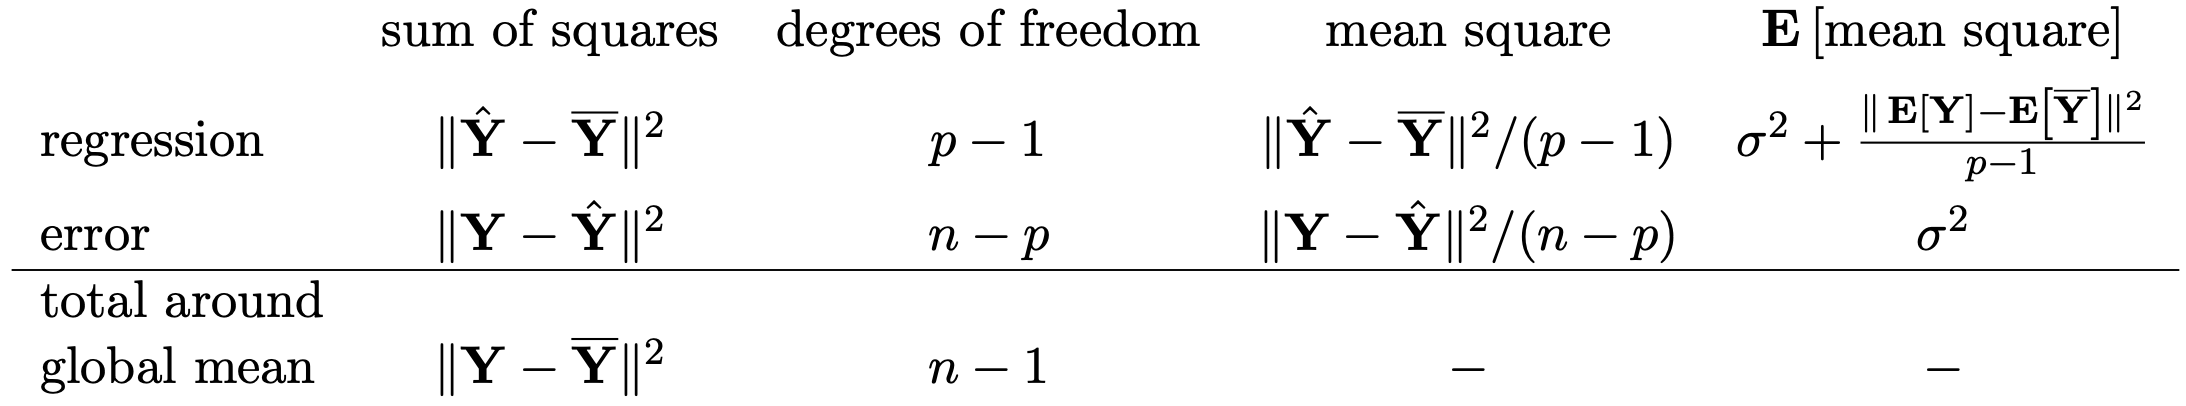
\includegraphics[width = 7cm]{ANOVA.png}
Under the null hypothesis $H_0:\beta = 0$ We have that:\\
$F=\frac{\Vert  \hat Y - \bar Y\Vert^2/(p-1)}{\Vert Y-\hat Y\Vert^2/(n-p)}\sim F_{p-1,n-p}$\\

\begin{codebox}{r}{P-Values \& ANOVA}
fit.smaller <- lm(y ~ x1)
# Anova uses RSS and DoF of largest (last) model, so
# use ascending order!
anova(fit.smaller, fit, fit.all)
# Overall F-Test
fit.empty <- lm(y ~ 1, data=...) # Empty model
anova(fit.empty, fit) # Compare models
# Alternative F-test
Ftest <- summary(fit)$fstatistic
pval <- 1 - pf(Ftest[1], df1=Ftest[2], df2=Ftest[3])
\end{codebox}


\textbf{R\textsuperscript{2} (Coefficient of determination):} the proportion of the total variation of the response $Y$ around its mean $\bar{Y}$ that is explained by the regression $\hat{Y}$ (via the ANalysis Of VAriance decomposition)
$R^2=\frac{||\hat{Y}-\bar{Y}||^2}{||Y-\bar{Y}||^2}=1-\frac{||Y-\hat{Y}||^2}{||Y-\bar{Y}||^2} = \frac{ESS}{TSS} = 1-\frac{RSS}{TSS}$

\begin{codebox}{r}{R squared}
RSE <- sqrt(sum(residuals(fit)^2)/(n-p))
RSS <- sum(res^2) # Residual sum of squares
TSS <- sum((y - mean(y))^2) # Total sum of squares
R.sq <- 1 - RSS / TSS
AdjR2 <- 1 - (RSS/(n-p))/(TSS/(n-1))
\end{codebox}

\subsection{Model selection}
To penalize large model we use Mallows statistic.\\
$C_P(\mathcal{M}) = n^{-1} RSS(\mathcal{M}) - \hat \sigma ^2 + 2n^{-1} \hat\sigma ^2\vert M\vert$. We can simply chose among all submodels the one with the best $C_p$ score, or, if it's too hard\\
\textbf{Forward stepwise:} 1) Fit $M_0$ 2) For $k=0,...,p-1$ fit all $p-k$ models with 1 additional predictor and select best (smallest RSS): $M_k$. 3) Select best among $M_0,....,M_p$ using CV or $C_p$. \\
\textbf{Backward stepwise:} 1) Fit $M_p$ (full model). 2) For $k=p,p-1,...,1$: fit all $k$ models that drop one perdictor in $M_k$. Choose best (smallest RSS): $M_{k-1}$. 3) Select best among $M_0,...,M_p$ using CV or $C_p$.
\begin{codebox}{r}{Stepwise methods}
library(leaps)
# Try all the submodels
regfit.full=regsubsets(Salary~., data=..., nvmax=19)
# Forward stepwise (method="backward" for backward)
regfit.full=regsubsets(Salary~., data=..., nvmax=19, method="forward")
\end{codebox}
\begin{codebox}{r}{Mallow Cp}
m <- regsubsets(y~., data=train, nvmax=10)
mo <- which.min(summary(m)$cp)
form <- as.formula(paste("y~",
  paste(names(coef(m,mo))[-1],collapse="+"), sep=""))
fit <- lm(form, data=test)
\end{codebox}

\subsection{R Diagnostic plots} \#1 Tukey-Anscombe Plot the points follow the line, else $E(\epsilon)=0$ violated. \#2 Q-Q Plot should follow line, else error not Gaussian (still all fine). \#3 Scale-Location: should be flat, else $\text{Var}(\epsilon_i)=\sigma^2$ violated (p-values wrong). \#4/\#5 Cook distance: shows if some data points have a larger impact on the fit than others (outliers). Note: can't detect if the residuals are correlated with these plots!



\textbf{Categorical Variables:} 
For two levels:$y_i = \beta_1 x_{i1}+...+\beta_p x_{ip} + \lambda d_{is} + \epsilon_i$ 
so if $i$ is in category, then $d_{is}=1$ else $d_{is}=0$. This acts as a different intercept ($E(y_i)-E(y_j)=\lambda$). If more categories, add more dummy variables.

\begin{codebox}{r}{Categ. var. by hand \& LOOCV}
a1 <- (levels(shelveloc)[2]==shelveloc)*1
lcv<-mean((residuals(fit)/(1-lm.influence(fit)$h))^2)
# Creating Categorical Variables
Carseats$High=ifelse(Carseats$Sales<=8,"No","Yes")
\end{codebox}

\textbf{Interaction:} dummy can also influence slope: add term $\delta d_i x_i$, can influence interaction between predictors: add term $\delta x_{i2} x_{i3}$, can influence other categorical variable: add term $\delta d_{i1}d_{i2}$.


\section{Confidence Intervals}
We find some CI of level $\alpha$, $\mathbb{P}(\in \text{CI}) = 1-\alpha$\\ 
\textbf{Coefficient}: $\beta_j \in [\hat \beta_j \pm \hat se(\hat \beta_j) \cdot t_{1- \alpha / 2, n-p}]$\\
\textbf{Expected value}: $\mathbb{E}[y\mid x] \in \left[x^T\hat{\beta} \pm \hat \sigma \sqrt{x^\top (X^\top X)^{-1} x} \cdot t_{1- \alpha / 2, n-p}\right]$\\
\textbf{Prediction interval}: $\hat y\mid x \in \left[x^T\hat{\beta} \pm \hat \sigma \sqrt{1 + x^\top (X^\top X)^{-1}x} \cdot t_{1-\alpha / 2, n-p}\right]$\\

\begin{codebox}{r}{Confidence Intervals}

confint(fit, level=0.95) # Automatic CI
# Manual CI (for intercept)
se.intercept <- summary(fit)$coef[1,2]
coef(fit)[1] - qt(.975, n-2)*se.intercept
coef(fit)[1] + qt(.975, n-2)*se.intercept
# Auto. Prediction CI (interval="c" for confidence)
predict(fit,data.frame(name=5),level=.95,interval="p")
# Manual Prediction CI
fitted <- fit$coef[1] + fit$coef[2]*x0
quant <- qt(.975,n-2) # Quantile of t distribution
sigma.hat <- sqrt(sum((fit$resid)^2/(n-2)))
X <- as.matrix(cbind(1,thuesen[,1]))
XtXi <- solve(t(X) %*% X)
X00 <- as.matrix(c(1,x0), nrow=2)
se <- sigma.hat * sqrt(t(X00) %*% XtXi %*% x00)
lower <- fitted - quant * se
upper <- fitted + quant * se
\end{codebox}

\subsection*{Bias Variance Trade-Off}
Expected Test MSE at $x_0$: $E[(\hat f(x_0) - y_0)^2] = \text{Bias}^2 (\hat f(x_0)) + \text{Var}(\hat f(x_0)) + \sigma^2$, where $\text{Bias}^2(\hat f(x_0)) = (E[\hat f(x_0)]-f(x_0))^2$.

\begin{codebox}{r}{Bias Variance Trade-Off of a Method}
Bias <- mean(EstimateUsingCV) - TrueValueSimulated
MSE <- Bias^2 + var(EstimateUsingCV)
\end{codebox}
\section{Non-parametric Regression}
We want to estimate $m(x)=\mathbb{E}[Y\mid X = x]$
\subsection{Nadaraya-Watson kernel method}
$\hat m(x)=\frac{\sum_iK((x-x_i)/h)Y_i}{\sum_iK((x-x_i)/h)}$. $h$ is the bandwidth. $K$ is the kernel function
\begin{codebox}{r}{Kernel method}
ksmooth(x, y, kernel = "normal", bandwidth = 0.2, x.points = x)
\end{codebox}
\textbf{Local bandwidth} To improve one idea is to have $h(x)$ depend on $x$ and not be the same everywhere.
\begin{codebox}{r}{Local bandwidth}
library(lokern)
lofit <- lokerns(cars$ speed, cars$ dist)
\end{codebox}
\textbf{Local polynomial:}
A piecewise degree $d$ polynomial with continuity in dimensions $0, ..., d-1$. Generally has $(k+1)(d+1)$ parameters and $k\cdot d$ constraints, so $k+d+1$ degrees of freedom. (e.g. \textbf{piecewise cubic} has $4(k+1)$ parameters and $3k$ constraint, so $k+4$ degrees of freedom. Basis functions: $h(x, \xi)=(x-\xi)_+^3$ ($0$ for all values $\leq \xi$). $y_i = \beta_0 + \beta_1 x_i + \beta_2 x_i^2 + \beta_3 x_i^3 + \gamma_1 h(x_i, \xi_1) + ... + \gamma_k h(x_i, \xi_k) + \epsilon_i$).\
\begin{codebox}{r}{Local polynomials}
model <- loess(y ~ x, span = 0.2971339), enp.target =df, surface="direct")# to predict non-train vals 
# span is the degree of smoothing, enp.target sets the df. Specify span OR enp.target, NOT both!
y_hat <- predict(model, newdata = x)
\end{codebox}
\textbf{Smoothing Splines:}\\ $G=\{ g:[a,b]\to \mathbb{R}: g'' \text{ exists and } \int_a^b g''(x)^2 dx < \infty \}$ is the class of functions to consider: $\hat g = \text{argmin}_{g\in G} \sum_{i=1}^n (y_i - g(x_i))^2 + \lambda \int_a^b g''(x)^2 dx$. Note: if $\lambda = 0$, $\hat g$ is any function in $G$ that passes through all data points. If $\lambda=\infty$, we get the least squares estimate. Shrunken version of natural spline with knots at $x_1, ..., x_n$. \\
\begin{codebox}{r}{Smoothing splines}
model <- smooth.spline(x, y, span = 0.2971339, df = 16, cv=T) #either specify span or df, not both!
y_hat <- predict(model, x = x)$y
\end{codebox}
\subsection{Degrees of freedom}
We define the hat matrix $\hat Y = \mathcal{S}Y$, for linear method. the degrees of freedom $df = \mathbf{tr}(\mathcal{S})$.\\
\begin{codebox}{r}{Compute hat matrix}
# Hat matrix "S.nw" to get degrees of freedom:
Id <- diag(nrow(data))
S <- matrix(0, nrow(data), nrow(data))
for (j in 1:nrow(data))
  S[, j] <- ksmooth(data[,"x"], Id[,j], x.point=data[, "x"], kernel="normal", bandwidth=4)$y
df <- sum(diag(S)))
\end{codebox}
\iffalse
\begin{codebox}{r}{Backfitting Algorithm for MLR}
backfit <- function(x, y, n, p, o, eps) {
  mu.hat <- mean(y) # Compute overall mean
  g <- matrix(0, nrow=n, ncol=p) # Initialize g
  converged <- FALSE
  while(!converged) {
    old.g <- g
    beta0.hat <- mu.hat 
    beta.hat <- numeric(p+1)
    for(i in o) { # o: order e.g. 1:p
      r <- y - mu.hat - rowSums(g[,-i])
      fit <- lm(r~x[,i])
      g[,i] <- fit$fitted
      beta0.hat <- beta0.hat + fit$coeff[1]
      beta.hat[1+i] <- fit$coeff[2]
    }
    if(max(colSums((old.g - g)^2)/colSums(old.g^2)) < eps) {
      converged <- TRUE
    }
    beta.hat[1] <- beta0.hat
  }
  return(beta.hat)
}
\end{codebox}
\fi
\section{Cross Validation}
Can be used for \textit{model assessment} (estimate test MSE) and \textit{model selection} (choose tuning parameters, variable selection). But not both at the same time (use double CV instead). \\
\textbf{Validation set:} split data into two halves, train on one, test on the other (most bias).
\textbf{k-Fold:} same, but with many folds. Try all folds for test and average metrics over the folds (in between). $\text{Var}(\hat {\theta_k}) = 1/K \cdot \hat {\text{Var}}(MSEs)$ \textbf{LOOCV:} extreme version where each data point is a fold (least bias, high variance since the datasets are correlated).\\
\textbf{LOOCV effiecent computation:} Assuming a linear model ($\hat Y = \mathcal{S}Y$) we have a fast way to find LOOCV. \\
$\text{LOOCV} = \frac{1}{n}\sum_{i=1}^n\left(\frac{Y_i-\hat m(X_i)}{1-\mathcal{S}_{ii}}\right)^2$\\
An historical approximation of this is GCV:\\
$\text{GCV} = \frac{1}{n}\sum_{i=1}^n\left(\frac{Y_i-\hat m(X_i)}{1-\frac{1}{n}\mathbf{tr}(\mathcal{S})}\right)^2$

\begin{codebox}{r}{Cross validation}
# Workaround for categorical variables
predict.regsubsets <- function(reg, new.data, id) {
  form <- as.formula(reg$call[[2]])
  mat <- model.matrix(form, new.data)
  coefi <- coef(reg, id=id)
  return(mat[,names(coefi)]%*%coefi)
}
n = nrow(data)
nfolds = 10
idx=seq(1:n)
idx <- idx[sample(n, replace=F)] # comment out for non-random
fold_indicator = cut(idx, breaks=nfolds, labels=F)
sse = 0
for(i in 1:nfolds){ 
  train <- data[i != fold_indicator,]
  test <- data[i == fold_indicator,]
  fit <- lm(y~x+I(x^2), data=train)
  preds <- predict(fit, test)
  sse = sse + mean((preds-test$y)^2 )
}
mse = sse / nfolds
mse
\end{codebox}

\section{Bootstrap}
Sample uniform from data points with replacement, compute bootstrapped estimator. For a large dataset $x_1, ..., x_n$ the probability that $x_1$ is contained in a random bootstrap dataset is: \\
$1-(1-1/n)^n \approx 2/3$ (for large $n$, limit goes to $1-1/e$).
\subsection*{Bootstrap Consistency}
For an increasing sequence $a_n$ (often $\sqrt{n}$) where $a_n^{-1}$ is the convergence rate of $\hat \theta_n$:
$\mathbb{P}(a_n(\hat \theta_n - \theta) \leq x) - \mathbb{P}^*(a_n(\hat \theta_n^* - \hat \theta_n) \leq x) \to^P 0$ as $n\to \infty$. This holds when $\sqrt{n}(\hat \theta_n - \theta)$ is asympt. normal. Allows to estimate $\text{Bias}(\hat \theta_n) = E[\hat \theta_n] - \theta$ by $E^*[\hat \theta^*_n] - \hat \theta_n$. Can also estimate $\text{Var}^*(\hat\theta_n)$ by $\text{Var}^*(\hat\theta^*_n)$ .
\subsection*{Bootstrap CI}
\textbf{Reversed Quantile CI:} (intelligent) $[\hat \theta_n - q_{\hat \theta^* - \hat \theta}(1- \alpha / 2), \hat \theta_n - q_{\hat \theta^* - \hat \theta}(\alpha / 2)]$ \textcolor{red}{(type="basic")}\\
\textbf{Normal Bootstrap CI:} Assume $\hat\theta_n$ to be asympt. normal: $\hat\theta_n \pm q_z(1-\alpha / 2)\hat{sd}(\hat\theta_n)$ where $z \sim \mathcal{N}(0,1)$ and $\hat{sd}(\hat\theta_n)=\sqrt {{\text{Var}(\hat\theta_n^*)}}$ \textcolor{red}{(type="norm")}\\ \textbf{Quantile Bootstrap CI:} (naive) not theoret. justified unless $\hat\theta_n$ is symm.:
$[q_{\theta_n^*}(\alpha / 2), q_{\theta_n^*}(1-\alpha / 2)]$ \textcolor{red}{(type="perc")}. Same as \textit{reversed quantile bootstrap CI} if $\hat\theta_n^* - \hat\theta_n$ is symm. around 0,\\ 
\textbf{Double bootstrap CI:} After we have a CI $I_\alpha$, we use a 2nd bootstrap estimate a $h(\alpha)\,s.t.\,\mathbb{P}(I_\alpha\hat\theta_n-\theta \ni \hat\theta_n-\theta) = 1-h(\alpha)$. Then we choose $\alpha'$ s.t. $h(\alpha')=\alpha$. Algo: 1) for each bootstrap iteration we take our bootstrap data and we run another round of bootstrap on that data to check weather the $\hat\theta^*$ fits in the CI. $h(\alpha)$ is the ratio of bootstrap iteration for which it fits inside\\
\textbf{Parametric Bootstrap:} We assume $X_1\dots X_n \sim P_\theta$. We estimate $\hat\theta$ then we draw bootstraps $X_1^*\dots X_n^*\sim P_{\hat\theta}$. More precise if the assumption is correct\\
\textbf{Regression bootstrap:} 
We do $Y_i^* = \hat m(x_i) + \epsilon_i$
\textbf{parametric:} 
$\epsilon_i \sim \mathcal{N}(0, \hat\sigma^2)$
\textbf{model-based:} 
$\epsilon_i \sim \hat P_{r}$, the empirical dist. of residuals
\begin{codebox}{r}{Bootstrap}
library(boot)
sample(c(1:n), n, replace=T) # bootstrap sample
# f statistics with args: (x, ind)
res.boot <- boot(data, f, R=100)# no. of bootstraps
res.boot$t0 # original estimates
res.boot$t # all the bootstrap estimates
# Example to find all confidence intervals
my_stat <- function(x, ind) {stat(x[ind])}
# Confidence intervals for variable i
boot.ci(res.boot, type= Look in red, index=i)
# Intervals by hand (t0: estimate, t: bootstrapped)
quantile.CI <- quantile(t,probs=c(0.025,0.975))
norm<-c(t0-qnorm(0.975)*sd(t),t0+qnorm(0.975)*sd(t))
reversed.CI <- t0-quantile(t-t0,probs=c(0.975,0.025))
\end{codebox}
% -*- root: Main.tex -*-
\section{Classification}
\subsection*{Loss-Functions}
True class: $y \in \{-1,1\}$, pred. $z \in [-1,1]$\\
Cross-entropy (log loss): ($y'=\tfrac{(1+y)}{2}$ and $z'=\tfrac{(1+z)}{2}$) $L(y',z') {=} -[y'log(z') {+} (1-y')log(1-z')]$ \\
Hinge Loss: $L(y,z) = max(0, 1-yz)$ \\
Perceptron Loss: $L(y,z) = max(0, -yz)$ \\
Logistic loss: $L(y,z) = log(1 + exp(-yz))$ \\
Square loss: $L(y,z) = \tfrac{1}{2}(1-yz)^2$ \\
Exponential loss: $L(y,z) = exp(-yz)$ \\
Binomial deviance: $L(y,z) = 1 + exp(-2yz)$ \\
0/1 Loss: $L(y,z) = \mathbb{I}\{sign(z)\neq y\}$ 
\subsection*{Probabilistic generative approach}
\( c^{*}=\argmin_c \mathcal{R}(c) \Rightarrow c^{*}(x) = \argmin_a \sum_y p(y\vert x)L(y,a)\) \\where \(p(y\vert x) \) is found from \(p(y,x)\) which is itself estimated somehow

\subsection*{Probabilistic discriminative approach}
Like Probabilistic generative approach but we estimate \(p(y\vert x)\) directly. \\\(p(y\vert x)=\argmax_w \mathcal{L}(\mathcal{Z}_{train}, w)= \argmax_w\sum_i\log{p(y_i\vert x_i, w)}\) where \(p(y\vert x; w) = \sigma(w^Tx + w_0)\). We can gradient descent on \(-\mathcal{L}\)

\subsection*{Discriminative approach}
Directly look for:\\ \(c^{*} = \argmin_c\hat{\mathcal{R}}(c, \mathcal{Z}_{train}) = \argmin_c \frac{1}{n}\sum_{i=1}^{n}L(y_i, c(x_i))\)

\subsection*{Percepton Algo} 
Find \(w, w_0\) s.t. \(y_iw^tx_i > 0 \;\forall i\). Gradient descent on \(L(y,c(x))=-yw^Tx\mathbb{I}_{\left(-\inf, 0\right)}\left(yw^Tx\right)\)\\
or {\scriptsize $L(y,c(x)) = \min_{\alpha_{1:n}} \sum_{i=1}^n \max  [0,- \sum_{j=1}^n \alpha_j y_i y_j x_i^T x_j ]$}

\subsection*{Fischer Discriminant}
\(w^{*} = \argmax_w \frac{w^TS_Bw}{w^TS_ww} = S_w^{-1}(\bar{x}_0-\bar{x}_1)\) where: \\
$S_B = (\bar{x}_0-\bar{x}_1)^T(\bar{x}_0-\bar{x}_1)$\\
\(S_w=\hat{Cov}(C_0) + \hat{Cov}(C_1)\) Sample variance matrixes for each cluster.\\
Fit a mixture of gaussians on $w^{*T}x$ insted of $x$

%\subsection*{Perceptron} 
%Gradient descent: $a(k+1) = a(k) - \eta(k)\nabla J(a(k))$ \\
%$J(a)\approx J(a(k))+\nabla J^T(a-a(k)) + \tfrac{1}{2}(a-a(k))^T H (a-a(k))$, $H{=}\frac{\partial^2 J}{\partial a_i \partial a_j}$ \\
%$2^{nd}$ order algorithm: $\eta_{opt} = \frac{\norm{\nabla J}^2}{\nabla J^T H \nabla J}$ \\
%Newton's rule: $a(k+1){=}a(k){-}H^{{-}1}\nabla J$\\
%Perceptron criteria: $J_p(a)=\sum_{\widetilde{x}\in\widetilde{\mathcal{X}}^{mc}} (-a^T \widetilde{x})$ \\
%Perceptron rule: $a(k+1)=a(k)+\eta(k)\sum_{\widetilde{x}\in\widetilde{\mathcal{X}}^{mc}} \widetilde{x}$ \\
%Perceptron convergence:$\left \| a(k+1)- \alpha \hat a \right \|^{2} = \left \| a(k)- \alpha \hat a \right \|^{2}  + 2(a(k)- \alpha \hat a)^{T} \tilde x^{k} + \left \| \tilde x^{k} \right \|^{2} \leq \left \| a(k)- \alpha \hat a \right \|^{2} -2\alpha \gamma + \beta ^{2}$
%where $\beta^{2} = max_{i}  \left \| \tilde x_{i \in \tilde X^{mc} } \right \| ^{2}$ and $\gamma = min_{i \in \tilde X^{mc} } (\hat a^{T} \tilde x_{i}) > 0 $ for $\alpha= \beta^{2} / \gamma$  then $k_{0}= \alpha^{2}\left \|\hat a \right \|^{2} / \beta^{2}=  \beta^{2}\left \|\hat a \right \|^{2} / \gamma^{2}$
%\subsection*{Bayesian Decision Theory}
%Est. cond. dist: $P(y|x,w) = Ber(\sigma(w^Tx))$\\
%Action set: $\mathcal{A} = \{ +1, -1\}$\\
%Cost fn: $C(y,a) = \{ 
%\begin{array}{lr}
%	c_{FP} \text{ , if $y=-1$ and $a=+1$}\\
%	c_{FN} \text{ , if $y=+1$ and $a=-1$}\\
%	0 \text{ , otherwise}
%\end{array}
%$
%The action that minimizes the expected cost is:\\
%$C_+ = \mathbb{E}_y[C(y,+1)|x] = P(y=+1|x) \cdot 0 + (P(y=-1)|x) \cdot %c_{FP}$\\
%$C_- = \mathbb{E}_y[C(y,-1)|x] = P(y=+1|x) \cdot c_{FN} + P(y=-1|x) \cdot %0$\\
%Predict +1 if $C_+ \leq C_-$

\section{Flexible regression}
Making some structural assumption, we estimate 
\begin{equation*}
    g(x)=\begin{cases}
    \mathbb{E}[Y\mid x]&\text{in regression}\\
    \text{logit}(\pi(x))&\text{in classification}
    \end{cases}
\end{equation*}
\subsection{Additive model}
In additive model we assume that \\
\begin{center}
    $g(x)=\mu +\sum_jg_j(x_j)$ {} {} {} {} {}    $\E[g_j(x_j)]=0\quad \forall j$\\
\end{center}
To find $\hat g_j$ we use \textbf{backfitting}:
Let $s_j: (u_1,...,u_n)^T \to (\hat u_1,...,\hat u_n)^T$ be a smoother (e.g. multiple linear regression). Order influences \#iterations\\
Initialize $\hat \mu = \frac 1 n \sum_{i=1}^n y_i$, \quad $\hat g_j = 0 \quad \forall j$\\
Do until convergence:\\
$\quad \text{for each } j=1,...p$:\\
$\quad \quad \hat g_j \gets s_j(y - \hat \mu \mathbb{1} - \sum_{k \neq j} \hat g_k)$\\
$\quad \quad \hat g_j \gets \hat g_j - \frac 1 n \sum_{i=1}^n \hat g_j(x_{ij}) \vec{1} $\\
\begin{codebox}{r}{GAM (generalized additive model)}
library(mgcv)
fitA <- gam(y ~ x_1+ x_2 + x_3, data = mydata)
predicted_y <- predict(fitA, testdata)
\end{codebox}

\subsection{MARS (Multivariate Adaptive Regression Splines)}
We make a regression with functions in $\mathcal{M}$. We start with $\mathcal{M}=\{h_0(\cdot)=1\}$. We then iteratively add functions in $\mathcal{M}$ in the form:
\begin{center}
$h_{\text{new},1-2}(x)=h_l(x)(\pm x_j\mp d)_+$
\end{center}
Where $h_l$ is in $\mathcal{M}$. We than prune back useless staff.
\begin{codebox}{r}{MARS}
library(earth)
Mfit <- earth(y ~ ., data = mydata, degree = 3) # no. of interactions
\end{codebox}
\subsection{Neural networks}
\begin{codebox}{r}{Neural nets in R}
library(nnet)
Nfit <- nnet(log.O3 ~ ., data = sc.ozone,
  size = 3,# n hidden layer
  decay = 4e-4,# regularization parameter
  skip=T)#add direct lin. params from input to output
  # other useful params: linout, softmax
\end{codebox}
\subsection{Projection pursuit regression}
\begin{center}
$g_{PPR}(x)=\mu + \sum_{k=1}^qf_k\left(\sum_{j=1}^p\alpha_{jk}x_j\right)$, where\\
$\Vert\alpha_k\Vert=1,\qquad\E\left[f_k\left(\sum_{j=1}^p\alpha_{jk}x_j\right)\right] =0,Var(f_k\left(\sum_{j=1}^p\alpha_{jk}x_j\right)) =1$
\end{center}
$f_k$ are called ridge functions. Backfitting to find $f_k$.
\begin{codebox}{r}{Projection pursuit regression in R}
fit <- ppr(y ~ . , data = dataset, nterms = 4)
#nterm is q (no. of terms to include in final model)
\end{codebox}

\subsection{CART (Classification and regression trees)}
The tree devides the domain in rectangles, in the end you have a piece-wise constant function. \\
$g_{\text{tree}}(x)=\sum_{r=1}^M\beta_r \mathbb{I}_{\mathcal{R}_m}(x)$\\
We can penalize larger tree to reduce variance. We choose the simplest model which is within standard error to the best one in cross-validation.
To fit we are greedy. \textbf{Pros} and \textbf{cons}:\\
$\bigcdot$ Highly flexible and interpretable\\
$\bigcdot$ Too simplistic, only piece-wise constant\\
$\bigcdot$ Prone to overfitting 
\begin{codebox}{r}{CART in R}
library(rpart)
rpart(y ~ ., data = data, control = rpart.control(cp = 0.0, minsplit = 30)) #minsplit: min no. of datapoints in a node to attempt a split
#cp = complexity factor, the R^2 must increase at least of a factor cp after split 
plotcp(tree) or printcp(tree) #estimate the best cp
prune.rpart(tree, cp=cp.opt) #to prune the tree
\end{codebox}
We are in the situation where $p>>n$.\\
\textbf{Ridge/Lasso regression:} We center and scale all the $x_i$ so that we can penalize all $\beta_i$ equally. In Ridge we penalize with $\Vert\beta\Vert_2^2$, in Lasso $\Vert\beta\Vert_1$.\\
\textbf{Elastic net} Mix of Ridge and Lasso, the regularization is\\
$\lambda_2\Vert\beta\Vert_2^2+\lambda_1\Vert\beta\Vert_1$. We call $\alpha = \frac{\lambda_2}{\lambda_1+\lambda_2}$. \\




\textbf{Adaptive lasso:} First you get an estimate of $\hat \beta$. Then we penalize more $\beta_i$ we think they are $0$, we set $w_j=\vert\beta\vert^{-\gamma}$. The regularization term will be $\lambda\sum_j w_j\vert\beta_i\vert$. \\
\text{Relaxed Lasso:} Like lasso but we use $\phi\lambda$ instead of $\lambda$ ($\phi \in [0,1]$). We then take out variables we don't need.\\
\textbf{Group Lasso:} Predictors are divided into $L$ groups of size $p_1, ..., p_L$ s.t. $\sum p_i = p$. $\hat\beta_\lambda^{gr.lasso}=\text{argmin}_\beta RSS(\beta)+\lambda \sum_{l=1}^L \sqrt{p_l} ||\beta||_2$ (if $L=p$, we get Lasso). Acts like Lasso on a group level. Useful if there are categorical variables with $>2$ categories (put all corresponding dummy variables in a group).\\

\begin{codebox}{r}{Ridge \& Lasso}
library(glmnet) # data must be a MATRIX!
grid <- 10^seq(from=10,to=-2,length=100)
ridge <- glmnet(x[train,], y[train], alpha=0, lambda=grid)
lasso <- glmnet(x[train,], y[train], alpha=1, lambda=grid)
# Coefficients for specific lambda_val
coef(lasso, s=lambda_val)
cv.glmnet(mm, y, alpha=0.5, nfolds=10)#For inbuilt CV
\end{codebox}
\section{Bagging-Boosting}
\subsection{Bootstrap Aggregating (Bagging)}
Bagging is a variance reduction technique.
We need a simple estimator $\hat g$ (for instance a tree). \\
1) We take $B$ bootstrap samples \\
2) For each bootstrap sample we train an estimator $\hat g_1,\dots,\hat g_B$. \\
3) Aggregation: $\hat g_{bag}(\cdot) = \frac{1}{B}\sum_{i=1}^B\hat g_i(\cdot)$ \\
\textbf{classification:} in this case we have majority voting (or we can average base estimator probs of being in each class)\\
\textbf{Subsample aggregating (Subagging):} Like Bagging but we just take subset of the dataset (without repetition) instead of bootstrapping. $m < n$ size of the subsets\\
\textbf{Out-of-Bag Error:}
Some bags have not trained on a particular sample. Can predict this only by the bags that have not been trained on it (should be $\sim 1/3$) for all samples and average to get a valid estimate for the test error. \\
\textbf{Random Forests:} 
Essentially bagged trees. Have $B$ bootstrap samples $\to$ create trees. They reduce dependence between tree estimates by only allowing a random subset of predictors at each split. Default: regression $p/3$, classification $\sqrt{p}$. (in R option mtry).
\begin{tabular}{|l|l|l|l|}
\hline
                 & Tree & Bagging & Random Forrest \\ \hline
Performance      & -    & +       & ++             \\ \hline
Computation      & +    & -       & +/-            \\ \hline
Interpretation   & +    & -       & -              \\ \hline
Out-of-bag error & -    & +       & +              \\ \hline
\end{tabular}
\begin{codebox}{r}{Random forest}
library(randomForest)
rf <- randomForest(y ~ . , data = mydata, mtry=p-1, importance = TRUE, ntree = 100)
# mtry: no. of features from which we chose a split. 
# if mtry = n_predictors then we have bagging trees
oob <- mean((rf$predicted-y.train)^2) #OOB Reg.
oob <- rf$err.rate #Classification
\end{codebox}
\subsection{Boosting}
Boosting is a bias reduction technique. We have $\hat g$ to be very simple estimator (stamp or small tree). We iteratively train a $\hat g$ predictor on the current model and then update the model: $f \gets f + \nu g$. ($\nu$ usually is $.1$) The other parameter is $M$.


%\section{Confidence Intervals}
We find some CI of level $\alpha$, $\mathbb{P}(\in \text{CI}) = 1-\alpha$\\ 
\textbf{Coefficient}: $\beta_j \in [\hat \beta_j \pm \hat se(\hat \beta_j) \cdot t_{1- \alpha / 2, n-p}]$\\
\textbf{Expected value}: $\mathbb{E}[y\mid x] \in \left[x^T\hat{\beta} \pm \hat \sigma \sqrt{x^\top (X^\top X)^{-1} x} \cdot t_{1- \alpha / 2, n-p}\right]$\\
\textbf{Prediction interval}: $\hat y\mid x \in \left[x^T\hat{\beta} \pm \hat \sigma \sqrt{1 + x^\top (X^\top X)^{-1}x} \cdot t_{1-\alpha / 2, n-p}\right]$\\

\begin{codebox}{r}{Confidence Intervals}

confint(fit, level=0.95) # Automatic CI
# Manual CI (for intercept)
se.intercept <- summary(fit)$coef[1,2]
coef(fit)[1] - qt(.975, n-2)*se.intercept
coef(fit)[1] + qt(.975, n-2)*se.intercept
# Auto. Prediction CI (interval="c" for confidence)
predict(fit,data.frame(name=5),level=.95,interval="p")
# Manual Prediction CI
fitted <- fit$coef[1] + fit$coef[2]*x0
quant <- qt(.975,n-2) # Quantile of t distribution
sigma.hat <- sqrt(sum((fit$resid)^2/(n-2)))
X <- as.matrix(cbind(1,thuesen[,1]))
XtXi <- solve(t(X) %*% X)
X00 <- as.matrix(c(1,x0), nrow=2)
se <- sigma.hat * sqrt(t(X00) %*% XtXi %*% x00)
lower <- fitted - quant * se
upper <- fitted + quant * se
\end{codebox}

\subsection*{Bias Variance Trade-Off}
Expected Test MSE at $x_0$: $E[(\hat f(x_0) - y_0)^2] = \text{Bias}^2 (\hat f(x_0)) + \text{Var}(\hat f(x_0)) + \sigma^2$, where $\text{Bias}^2(\hat f(x_0)) = (E[\hat f(x_0)]-f(x_0))^2$.

\begin{codebox}{r}{Bias Variance Trade-Off of a Method}
Bias <- mean(EstimateUsingCV) - TrueValueSimulated
MSE <- Bias^2 + var(EstimateUsingCV)
\end{codebox}
%\section*{Permutation Test}
Non-parametric, simple model that works with any test statistic. P-values and type I error control exact/approximate (not asymptotic), but needs computational power and not everything can be modeled in this way (e.g. individual coefficients in LR) \\
{1. Pick a test stat. that measures some difference between groups}\\
{2. Consider all possible permutations (or randomly permute) to obtain a permutation distribution.}\\
{3. Compare observed value to permutation distribution}\\

\subsection*{Wilcoxon Test}
Non-parametric, unpaired, robust test. $H_0: F_1 = F_2$, $H_A: F_1 $ shifted compared to $F_2$. Compute ranks of randomly switched sign (different group assignment), reject $H_0$ if observed rank over critical value of rank distribution.

\begin{codebox}{r}{Permutation Test \& Wilcoxon Signed Rank Sum Test}
# Permutation test
fit <- lm(y~X)
obsF <- summary(fit)$fstatistic[1]
res.f <- rep(NA, 10000)
for (i in 1:10000){
  y <- y[sample(1:nrow(X), nrow(X))]
  fit.tmp <- lm(y~X)
  res.f[i] <- summary(fit.tmp)$fstatistic[1]
}
pval<-(sum(obsF<=res.f,na.rm=T)+1)/(length(res.f)+1)
# Permutation Wilcoxon Signed Rank Sum Test
diff <- immer$Y1 - immer$Y2
V.obs <- sum(rank(abs(diff)) * (diff > 0))
V <- numeric(100000)
for(i in 1:100000){
  perm<-diff * sample(c(1,-1),nrow(immer),replace=T)
  V[i] <- sum(rank(abs(perm)) * (perm > 0))
}
p.value <- table(V >= V.obs)["TRUE"]/length(V)
# Automatic
wilcox.test(diff, alternative = "greater")
\end{codebox}

% Maybe drop this
%\subsection*{Exercise Wilcoxon}
%Let $X_1,...,X_m~F_X$ and $Y_1,...,Y_m~F_Y$ be independent. $H_0: F_X=F_Y$, $H_A: F_X(x) = F_Y(x-a) \  \forall x$ and $a>0$. Let $D_i = X_i - Y_i, i \in [1,m]$. Show that $H_0$ and $H_A$ can be written as $H_0: $ the distribution of $D$ is symmetric around $a=0$, $H_A$ the distribution of $D$ is symmetric around $a>0$. \\
%We show that the distribution of $D$ is symmetric around $a$: $P(D-a \leq d) = P(-(D-a) \leq d)$. We have $P(D-a \leq d) = P(D \leq d + a) = \int P(X-Y \leq d+a |Y=y) f_Y(y) dy = \int P(X-y \leq d+a) f_Y(y) dy = \int P(X \leq d+a+y) f_Y(y) dy = \int F_X(d+a+y)f_Y(y)dy$ We get the same when exchanging $X$ and $Y$: $P(-(D-a)\leq d) = P(-D \leq d-a) = P(Y-X \leq d-a) = \int F_Y(d-a+x)f_X(x)dx$. \\
%We can use that $F_X(x)=F_Y(x-a)$ and $f_X(x)=f_Y(x-a)$ to show: $\int F_X(d+a+y)f_Y(y)dy = \int F_Y(d+a+y-a)f_X(y+a)dy = \int F_Y(d+y)f_X(y+a)dy = \int F_Y(d-a-x)f_X(x)dx$
%\section*{Multiple Testing}
\begin{tabular}{l|l|l|l}
 & \textbf{$\mathbf{H_0}$ true} & \textbf{$\mathbf{H_A}$ true} &  \\ \hline
$\mathbf{H_0}$ \textbf{not reject.} & $U$ true neg. & \begin{tabular}[c]{@{}l@{}}$T$ false neg.\\ Type II error\end{tabular} & $m-R$ \\ \hline
$\mathbf{H_0}$ \textbf{reject.} & \begin{tabular}[c]{@{}l@{}}$V$ false pos.\\ Type I error\end{tabular} & $S$ true pos. & $R=V+S$ \\ \hline
 & $m_0$ & $m-m_0$ & $m$
\end{tabular}
Capital letters represent RV. Only $R$ is observable. $m$ is fixed and known, $m_0$ is fixed and unknown. If $m_0=m$ then \textit{global null}. \\
$P(\textit{type I error}) = P(\textit{rejecting } H_0 \textit{ when } H_0 \textit{ is true}) = \alpha$ \\
$P(\textit{type II error}) = P(\textit{not rejecting } H_0 \textit{ when } H_A \textit{ is true}) = \beta$ \\
\textbf{Power of a test} $1-\beta$ 
\textbf{False discovery proportion (FDP):} $Q=V/R$ (note: $V/R=0$ if $V=R=0$) 
\textbf{False discovery rate (FDR):} $E(Q)$ Expected proportion of false discoveries among all disc. \textbf{Family wise error rate (FWER):} $P(V\geq 1)$ Prob. of making one or more false discoveries. Note: controlling the FWER is more strict than controlling the FDR: if $V\geq 1$, then $Q=V/R \leq 1$ and if $V=0$, then $Q=V/R=0$. So $\mathds{1}_{\{V\geq 1\}}\geq Q$: $\text{FWER}=P(V\geq 1)=E[\mathds{1}_{\{V\geq 1\}} \geq E[Q] = \text{FDR}$. If $m=m_0$ then $\text{FWER}=\text{FDR}$.

\subsection*{Bonferroni Correction}
Idea: $\text{FWER}=P(V\geq 1)=P(\textit{at least one false rejection among tests }\allowbreak T_1,...,T_m)=P(\cup_{i=1}^m\{\textit{false rejection in test }T_i\}) \leq \sum_{i=1}^m P(\{\textit{false rej.} \allowbreak \textit{ in test}\}) \leq \sum_{i=1}^m \alpha = m\cdot \alpha$ so we set the signif. level of individual tests to $\alpha' =\alpha /m$, then $\text{FWER}\leq m\alpha' =\alpha$. Power: if the tests are indep. and $m=m_0$ then $\text{FWER}=1-(1-\alpha)^m$ which is $\approx \alpha\cdot m$ for small $\alpha$ and moderate $m$. If the tests are correlated: too conservative.

\subsection*{Benjamini-Hochberg}
Let $p(1)\leq p(2) \leq ... \leq p(m)$ be ordered p-values. Let $i_0$ be the largest $i$, s.t. $p(i)\leq q\cdot i / m$. Reject all $H_{(i)}$ with $i\leq i_0$. For independent test statistics (or p-values) this controls the $\text{FDR}$ at level $q$, i.e. $\text{FDR}=q\cdot m_0 / m \leq q$. 
\subsection*{Westfall Young Permutation Procedure}
Provides \textit{weak control of the FWER} (i.e. under the global null). \\
Given a data $X \in \mathbb{R}^{n\times (m+1)}$ size and $y\in \{0,1\}^n$. If $m=m_0$ then one can permute the y-values:\\
1. Repeat many times: premute y-cols, do a two sample test (e.g. Wilcoxon) for each $x_j$ col. (comparing $x_j[y==1]$ and $x_j[y==0]$). Let $p_j$ for $j=0,...,m$ be the corresp. p-value. Store $\min(p_1,...,p_m)$.\\
2. Set $\delta$ to the empirical $\alpha$-quantile of the permutation distribution of $min(p_1,...,p_m)$. \\
3. Reject any null hypothesis where the two-sample test on the original data has p-value $\leq \delta$.\\

\begin{codebox}{r}{Westfall Young Permutation Procedure}
nr.sim <- 1000
min.p.values <- numeric(nr.sim)
for(sim in 1:nr.sim) {
  y_perm = sample(y, length(y), replace = FALSE)
  min.p.values[sim] <- min(apply(x, 2, function(j) chisq.test(x = j, y = y_perm)$p.value))
}
delta <- quantile(min.p.values, probs = 0.05)
table(p.values < delta)
\end{codebox}
%\section*{K Nearest Neighbors}
Non-parametric method: $\hat f(x)=1/k \sum_i yi$ where $y_i$ are the $k$ nearest neighbors of $x$. If $k$ is larger has less variance, more bias. If $k$ is smaller has more variance, less bias.
Fails if there are lots of useless predictors.

\begin{codebox}{r}{KNN}
library(kknn)
dfTrain=data.frame(y=Ytrain,x=Xtrain)
dfTest=data.frame(x=Xtest)
fit.kknn <- kknn(y ~ ., dfTrain,dfTest,k=8)
predTest=predict(fit.kknn) # predictions on dfTest
library(class) # Alternative library for knn
knn(train, test, k=5)
\end{codebox}
%\section*{Tree Based Methods}
$y_i = \sum_{r=1}^M \beta_r \mathds{1}_{x_i\in R_r} + \epsilon_i$. Where $R_1, ..., R_M$ are regions (we limit ourselves to rectangular regions). \\
\textbf{Recursive Binary Splitting:} Greedy method to find the regions: For all predictors find the best cutting point, then take the cutting point that minimizes the error $\sum_{i: x\in R_1} (y_i - \bar y_{R_1})^2 + \sum_{i: x \in R_2} (y_i - \bar y_{R_2})^2$. Stop when region contains less than 5 elements. \\
\textbf{Pruning:} A deep tree $T_0$ can overfit. Pruning is a possible solution: For $\alpha >0$: find $\text{argmin}_{T\subset T_0} err(T) + \alpha |T|$. ($\alpha$ is tuning parameter, find via CV). \\
\textbf{Classification Trees:} At each split, try to improve node purity measured by gini index: $I(D) = [\frac{n_L}{n} I(D_L) + \frac{n_R}{n} I(D_R)] > 0$ where the subtrees are $I(D_R) = \hat p (1-\hat p)$ where $\hat p = \frac{\#yes}{\#yes + \#no}$. Can predict class probability $\hat p_k(x) = \textit{proportion of observations with class }k\textit{ in leaf node that contains }x$.


\begin{codebox}{r}{Using Trees}
train.ind <- sample(n, round(n/2), replace = FALSE)
train.data <- Carseats[train.ind,]
test.data <- Carseats[-train.ind,]
# Create and plot tree
cs.tree <- tree(Sales ~ . , train.data)
plot(cs.tree)
text(cs.tree, pretty=1)
# Predict using tree
test.pred <- predict(cs.tree, test.data)
(MSE <- mean((test.data$Sales - test.pred)^2))
# Prune tree
cv.carseats = cv.tree(cs.tree, FUN=prune.tree)
best.size <- cv.carseats$size [which.min(cv.carseats$dev)]
pruned.tree <- prune.tree(cs.tree, best = best.size)
\end{codebox}
\begin{codebox}{r}{R-Help}
#argmax_per row
probs <- predict(tree, newdata = data)
pred<-colnames(probs)[max.col(probs)]
# Workaround for automatic dimension collapse
matrix(X[test.fold,], nrow=n/k)
# Test if an element is in a list
if ("X1" %in% names(coef(m,mo)))
# Fit distribution to data vector
library(MASS)
fit.gamma <- fitdistr(boogg, "gamma")
thuesen <- thuesen[!is.na(thuesen[,2]),] # Remove NA
data_comp <- data[complete.cases(data),]
scaled.dat <- scale(dat) # Standardize data
apply(X, d, func) #apply func to all rows(d = 1) or cols(d = 2) of matrix X
sapply(X, func) #apply func to elems in the list X
rep(x=0, times=100) # Create empty vector
dataset[,"logX"] <- log(dataset[,"X"])# Log transform
# Order dataframe accordind to column x1
dfOrdered <- df[order(df$x1, decreasing = F),]
data.matrix(df) # Dataframe to Matrix
myList <- numeric(n) # Initialize empty list size n
y <- X %*% beta #matrix product operator
i <- a %% c #modulo operator 
# Predict help to get model specific params
?predict.loess # Replace 'loess' with wanted function
ls("package:lokern") # list of methods in package
\end{codebox}



\end{multicols*}
\end{document}